\section{Edge Detection}
The edge detection problem aims at identifying the \emph{edges} inside an image; this requires a proper definition of \say{edge}, which often depends on the method used to compute it. In general, an edge is a place where the intensity of the image changes abruptly. 

The edge detection problem is a fundamental problem in computer vision, as it is the first step in many image processing tasks. The main motivation behind edge detection is the idea that the edges of an image contain important information about the structure of the objects in the scene. If the brightness of an image changes abruptly, it is likely that other properties of the image also change abruptly at that point, and specifically higher-level properties. Edges define the boundaries of objects in the image; they are caused by change of texture, color, depth, or illumination, which all are important cues for the semantic interpretation of the image.

\subsection{Gradient-based edge detection}
Intuitively, an edge is a discontinuity of intensity in some direction; like explained previously, it could be detected by looking for place where the derivatives of the iamge have large values.

Gradient-based edge detectors run into three major issues:
\begin{description}
    \item[Change of scale] The gradient magnitudes at different scales are different: which one should we choose? This reflects a fundament problem in computer vision, which is the necessity to select a threshold under which edges are \say{too small} to be considered.
    \item[Thick countours] The gradient magnitude is large along thick trails: how do we identify the significant points?
    \item[Continuity] Simple edge detection algorithms will produce non-continuous lines, which does not fit our high-level understanding of edges. How do we link the relevant points up into curves?
\end{description}

Another way to detect an extremal first derivative is to look for a null second derivative. In practice, applying a Laplacian method always require smoothing with a Gaussian kernel first. The method goes as follows: smooth the image, apply the Laplacian, and mark the zero points where there is a sufficiently large derivative -- that is enough contrast.

\subsection{The Canny edge detector}
\subsubsection{Introduction}
The Canny edge detector is a multi-step edge detection algorithm, providing a good trade-off between the three issues mentioned above. Instead of simply thresholding the gradient magnitude -- which would lead to thick contours and discontinuous lines -- the Canny edge detector track edges using a process called \emph{hysteresis}.

The starting point of Canny's results is the observation that gradient magnitude does enhance the edges, but runs into two main issues:
\begin{itemize}
    \item using a single threshold either leads to too many edges, or too few edges;
    \item even if we find a good threshold, the edges remain poorly localized, i.e. too thick.
\end{itemize}
Therefore, Canny's edge detector uses two standard tools to address these issues, \emph{non-maximum suppression} and \emph{hysteresis}.

\subsubsection{Non-local maxima suppression}
The goal of Non-Maximum Suppression (NMS) is to thin the edges; the idea is to keep only the pixels that correspond to a maximum in one of the directions of the gradient. If in all directions, the pixel is not a maximum, then it is likely to be a thick contour, and should be removed. Conversely, if the pixel is a maximum in one direction, it is likely to be at the center of the edge stroke, and should be kept.
\begin{figure}[H]
    \centering
    \begin{minipage}{.4\textwidth}
        \centering
        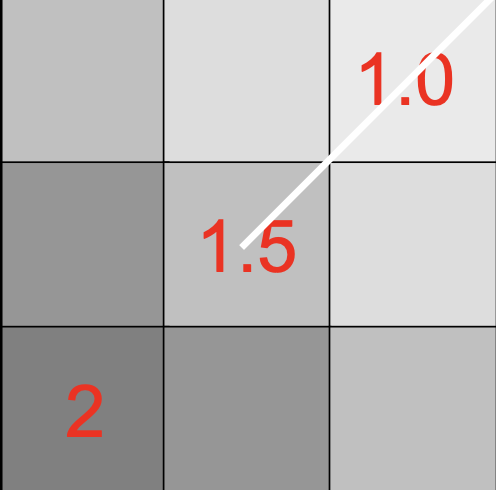
\includegraphics[width=.6\textwidth]{edge-detection/nms-1.png}
        \caption*{Gradient magnitude at center is lower than a neighbor}
    \end{minipage}
    \begin{minipage}{.4\textwidth}
        \centering
        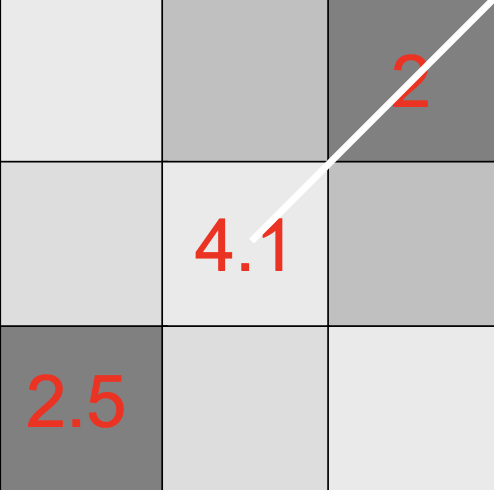
\includegraphics[width=.6\textwidth]{edge-detection/nms-2.png}
        \caption*{Gradient magnitude is a local maximum}
    \end{minipage}
\end{figure}
This creates a mask of the image, where only the local maxima are kept. Applying this mask to the gradient magnitude image will therefore thin the edges.
\begin{figure}[H]
    \centering
    \begin{minipage}{.3\textwidth}
        \centering
        
\includegraphics[width=.8\textwidth]{edge-detection/edge-1.png}
    \end{minipage}
    \begin{minipage}{.3\textwidth}
        \centering
        
\includegraphics[width=.8\textwidth]{edge-detection/edge-2.png}
    \end{minipage}
    \caption{The left image shows the gradient magnitude of an image; on the right, the mask provided by NMS and its application to the gradient.}
\end{figure}

\subsubsection{Hysteresis thresholding}
As stated previously, lower thresholds keep important details, but also keep a lot of noise; higher thresholds remove the noise, but also remove important information about the edges. The idea of hysteresis thresholding is to use two thresholds, a lower and an upper one, to keep only the pixels that are above the upper threshold, or connected to a pixel above the upper threshold. This allows to keep the important details, while removing the noise (i.e. the pixels that are not connected to the edges). Hysteresis also tend to produce continuous edges, since we track the edges by following the pixels that are connected to the edges.
\begin{figure}[H]
    \centering
    \begin{minipage}{.6\textwidth}
        \centering
        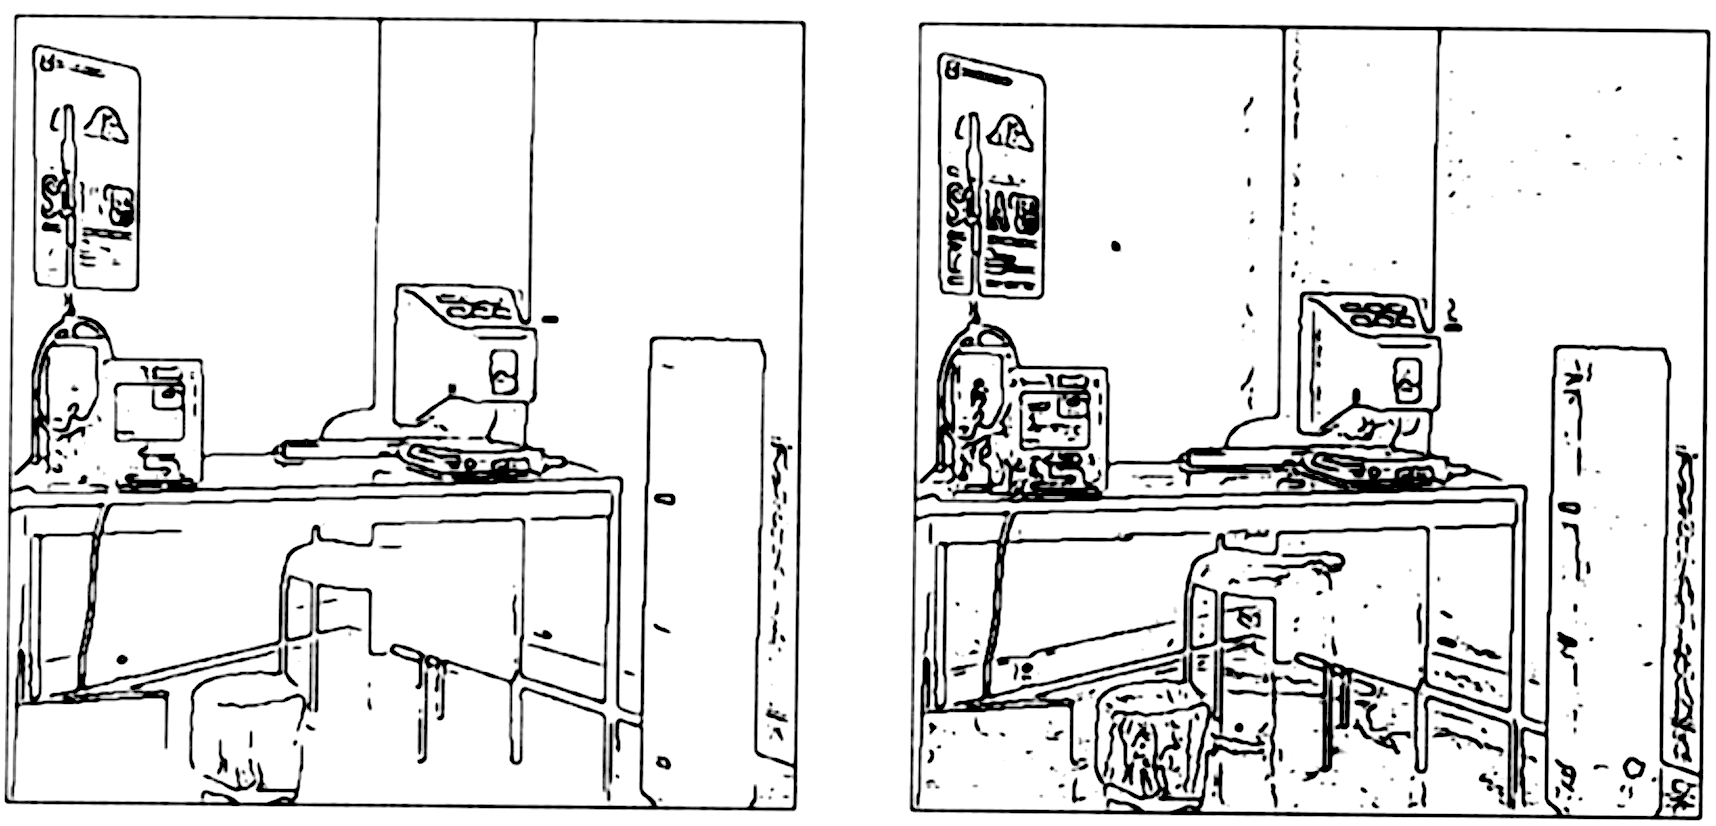
\includegraphics[width=.9\textwidth]{edge-detection/thresholds.png}
        \caption*{Two thresholds: $t=15$ and $t=5$}
    \end{minipage}
    \begin{minipage}{.3\textwidth}
        \centering
        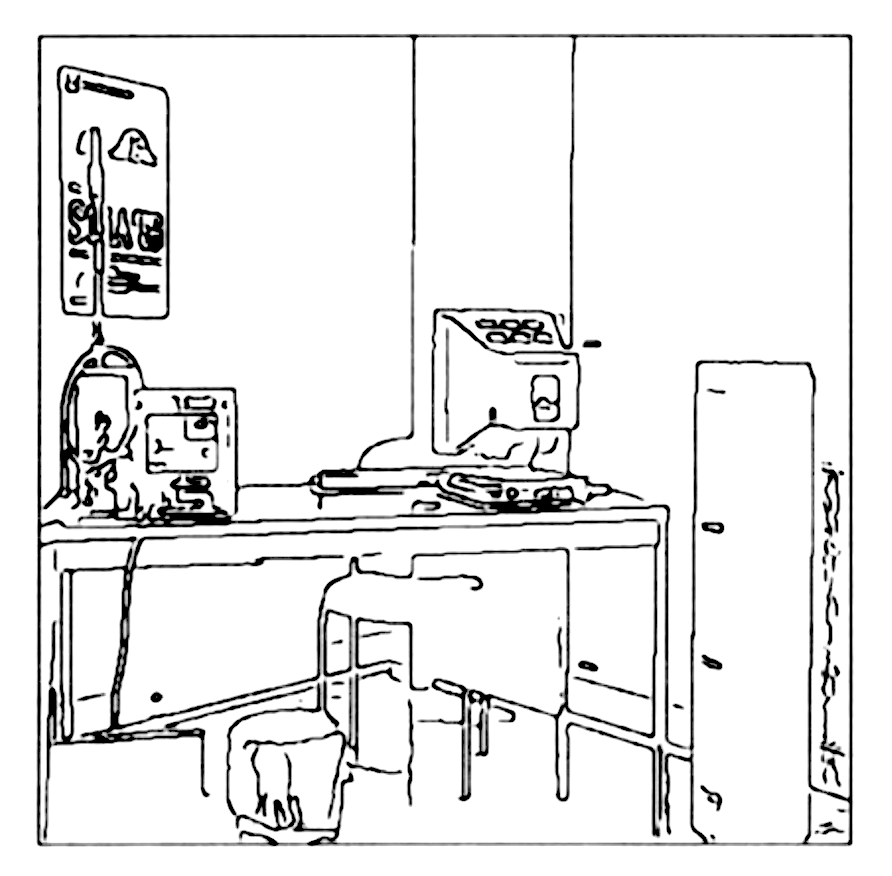
\includegraphics[width=.9\textwidth]{edge-detection/hysteresis.png}
        \caption*{Hysteresis thresholding}
    \end{minipage}
\end{figure}

Hysteresis thresholding can be implemented using a depth-first search algorithm, which will track the pixels connected to the edges. The algorithm goes as follows:
\begin{enumerate}
    \item Keep a set $E$ of the edges for which you have to visit neighbours;
    \item Initialize $E$ with the edges corresponding to the most discriminative threshold;
    \item Until $E$ is empty:
    \begin{itemize}
        \item Extract an edge $e$ from $E$; if $e$ has already been visited, skip it;
        \item For each neighbour $e'$ of $e$:
        \begin{itemize}
            \item If $e'$ is a considered edge using the less discriminative threshold, add it to the output edges and to $E$
            \item Otherwise, skip it
        \end{itemize}
    \end{itemize}
\end{enumerate}

\subsubsection{The algorithm}
Putting all the steps together, the Canny edge detector goes as follows:
\begin{enumerate}
    \item Compute $x$ and $y$ derivatives of the image $I$:
    \begin{equation*}
        I_x = G^x_\sigma * I \quad \text{and} \quad I_y = G^y_\sigma * I
    \end{equation*}
    \item Compute the magnitude of the gradient at every pixel:
    \begin{equation*}
        |\nabla I| = \sqrt{I_x^2 + I_y^2}
    \end{equation*}
    \item Eliminate the pixels that are not local maxima of the magnitude in the direction of the gradient:
    \begin{equation*}
        |\nabla I|_{\text{NMS}} = \text{NMS}(|\nabla I|)
    \end{equation*}
    \item Apply hysteresis thresholding to the image:
    \begin{equation*}
        \text{Canny}(I) = \text{Hysteresis}(|\nabla I|_{\text{NMS}}, t_h, t_l)
    \end{equation*}
\end{enumerate}